\subsubsection*{Analysis}
\begin{tabular}{@{}l l}
\textbf{Scope}:&
The AuctionHouse\textsuperscript{TM} automated administration system\\
\textbf{Level}:&
User goal\\
\textbf{Primary Actor}:&
Purchasing Agent, Auctioneer, Secretary\\
\textbf{Stakeholders and Interests}:&
\begin{tabular}[t]{@{}l}
Purchasing Agent, Auctioneer, Secretary: wants to update ??? an item's\\
parameters ??? quickly and easly
\end{tabular}\\
\textbf{Preconditions}:&
Actor is identified and authenticated.\\
\textbf{Postconditions}:&
\begin{tabular}[t]{@{}l}
The item has been updated on the system, or a failure was returned.\\
The updates to the item's parameters are (or will become) visible for potential\\
 buyers and the otherwise authorized.
\end{tabular}\\
\textbf{Special requirements}:&
\begin{tabular}[t]{@{}l}
The current parameters of an item and a list of future auction dates needs\\
to available in the system.
\end{tabular}\\
\textbf{Frequency of occurence}:&
\begin{tabular}[t]{@{}l}
Daily. Dependent on how many mistakes the purchasing agent makes when\\
entering an item, how often a seller wishes to change something about their\\
items (via the secretary) and how many auctions there are where auctioneers\\
 need to mark the item as sold or junk.
\end{tabular}\\
\end{tabular}\\\\
\textsl{Main Success Scenario}
\begin{enumerate}[noitemsep]
	\item The user starts the update item transaction, with all parameters to be updated ready.
	\item The system provides the user with the current parameters of the item that they are authorised to edit.
	\item The user provides the updated parameters. The parameters that can be updated are:
	\begin{itemize}[noitemsep]
		\item The amount of the item available
		\item The type of item
		\item A description
		\item If the item possesses any antiquarian value
		\item A minimum price decided by the owner
		\item The date when brought in
		\item Name and address of the owner plus identification
		\item Planned auction date
		\item Distinguishing features
	\end{itemize}
	\item The system updates the item with the given parameters.
	\item The system returns to the user whether it was successful.
\end{enumerate}
\textsl{Extensions}
\begin{itemize}[noitemsep]
	\item If unsucessful, the system database remains unchanged; no item or other parameters was added or changed.
\end{itemize}
\textsl{System Sequence Diagram}
\begin{figure}[H]
	\centering
	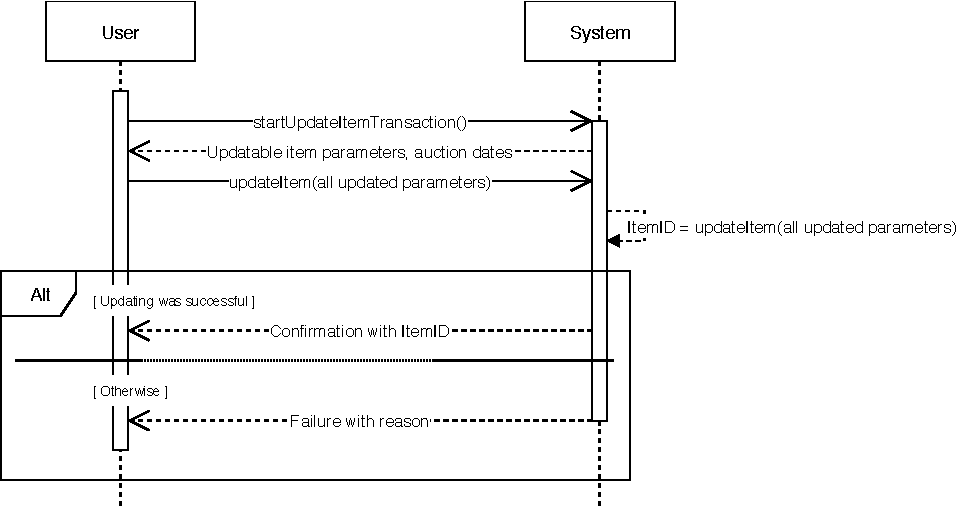
\includegraphics[scale=1]{SD-bb-update.pdf}
	\caption*{Interactions displayed in a System Sequence Diagram in blackbox format}
\end{figure}